\chapter{Needle Algorithm}
\label{sec:analysis}

\begin{algorithm}[t]
\DontPrintSemicolon
\KwData{$proxies$, $n$, $s=\lfloor{n/g}\rfloor$}
\KwResult{One of $\{px_1, px_2\}$}
\Begin{
    $window \longleftarrow (start, end)$\;
    \uIf{$move > 1$}{
        \tcc*[l]{a giant step around the proxy ring}

        $start \longleftarrow (start + s)$ \% $n$\;
        $end \longleftarrow (end + s)$ \% $n$\;
        $move \longleftarrow 0$
    }
    
    $move \longleftarrow move + 1$\;
    
    $sublist \longleftarrow (proxies$ $[start, end])$\;

    $px_1 \longleftarrow$ random$(sublist)$\;
    $px_2 \longleftarrow$ random$(sublist)$\;
    $l_1 \longleftarrow$ $load(px_1)$\;
    $l_2 \longleftarrow$ $load(px_2)$\;

    \uIf{$l_1 == l_2$}{
        return $px_1$\;\tcc*[r]{break a tie}
    }
    \uElseIf{$l_1 > l_2$}{
        return $px_1$\;\tcc*[r]{$px_1$ is heaviest loaded}
    }
    return $px_2$\;\tcc*[r]{$px_2$ is heaviest loaded}
    
}
\caption{Needle Algorithm \label{needle}}
\end{algorithm}

We present a new algorithm, the \emph{needle} algorithm, and compare it to two well-known algorithms, uniform random and power of 2 choices, as well as Tor's bridge distribution scheme, in order to contrast their respective trade-offs and suitability under differing system goals. The primary goal of the needle algorithm is to preserve some proxies from within the larger list of $n$ proxies. Another goal is to maintain practical load balancing for the majority of the proxies. It achieves these goals by breaking the list of proxies into sublists. It moves through the proxies jumping from sublist to sublist, referred to as \texttt{GIANTSTEPS} or $g$. These steps isolate some proxies from distribution.\footnote{Those readers familiar with the algorithmic composition techniques of jazz chord progression may draw a parallel from the restriction of proxies to the restriction of notes in a key change. These are reminiscent of Coltrane's Giant Steps \cite{lateef1981repository}.} The algorithm has the following parameters:
    \begin{itemize}
        \item $proxies$: a sorted list of proxies ordered by load
        \item $n$: the total number of proxies
        \item $g$: the number of steps around the proxy ring
        \item $s$: the number of proxies in each $g$ step
        \item $move$: move to the next step 
        \item $px_1, px_2$: two randomly selected proxies from within the $sublist$ of the current step $g$, sampled with replacement
    \end{itemize}

The algorithm selects two proxies uniform randomly in each giant step $g$. Using reverse power of 2 choices, it then chooses the \textit{heavier loaded} proxy and returns this proxy to the collector. (Note that the standard power of d choices algorithm chooses the lighter loaded proxy.) The step begins at the bottom of the list of proxies and is moved step-wise around the list eventually wrapping so that all proxies have an opportunity to be selected, shown in Figure \ref{fig:giantstepring}.

%%%%%%%%%%%%%%%%%%%%%%%%%%%%%%%%%%%%%%%%%%%%%%%%%%%%%%%%%%%%%%%%%%%%%%
\begin{figure*}[h!]
\centering
     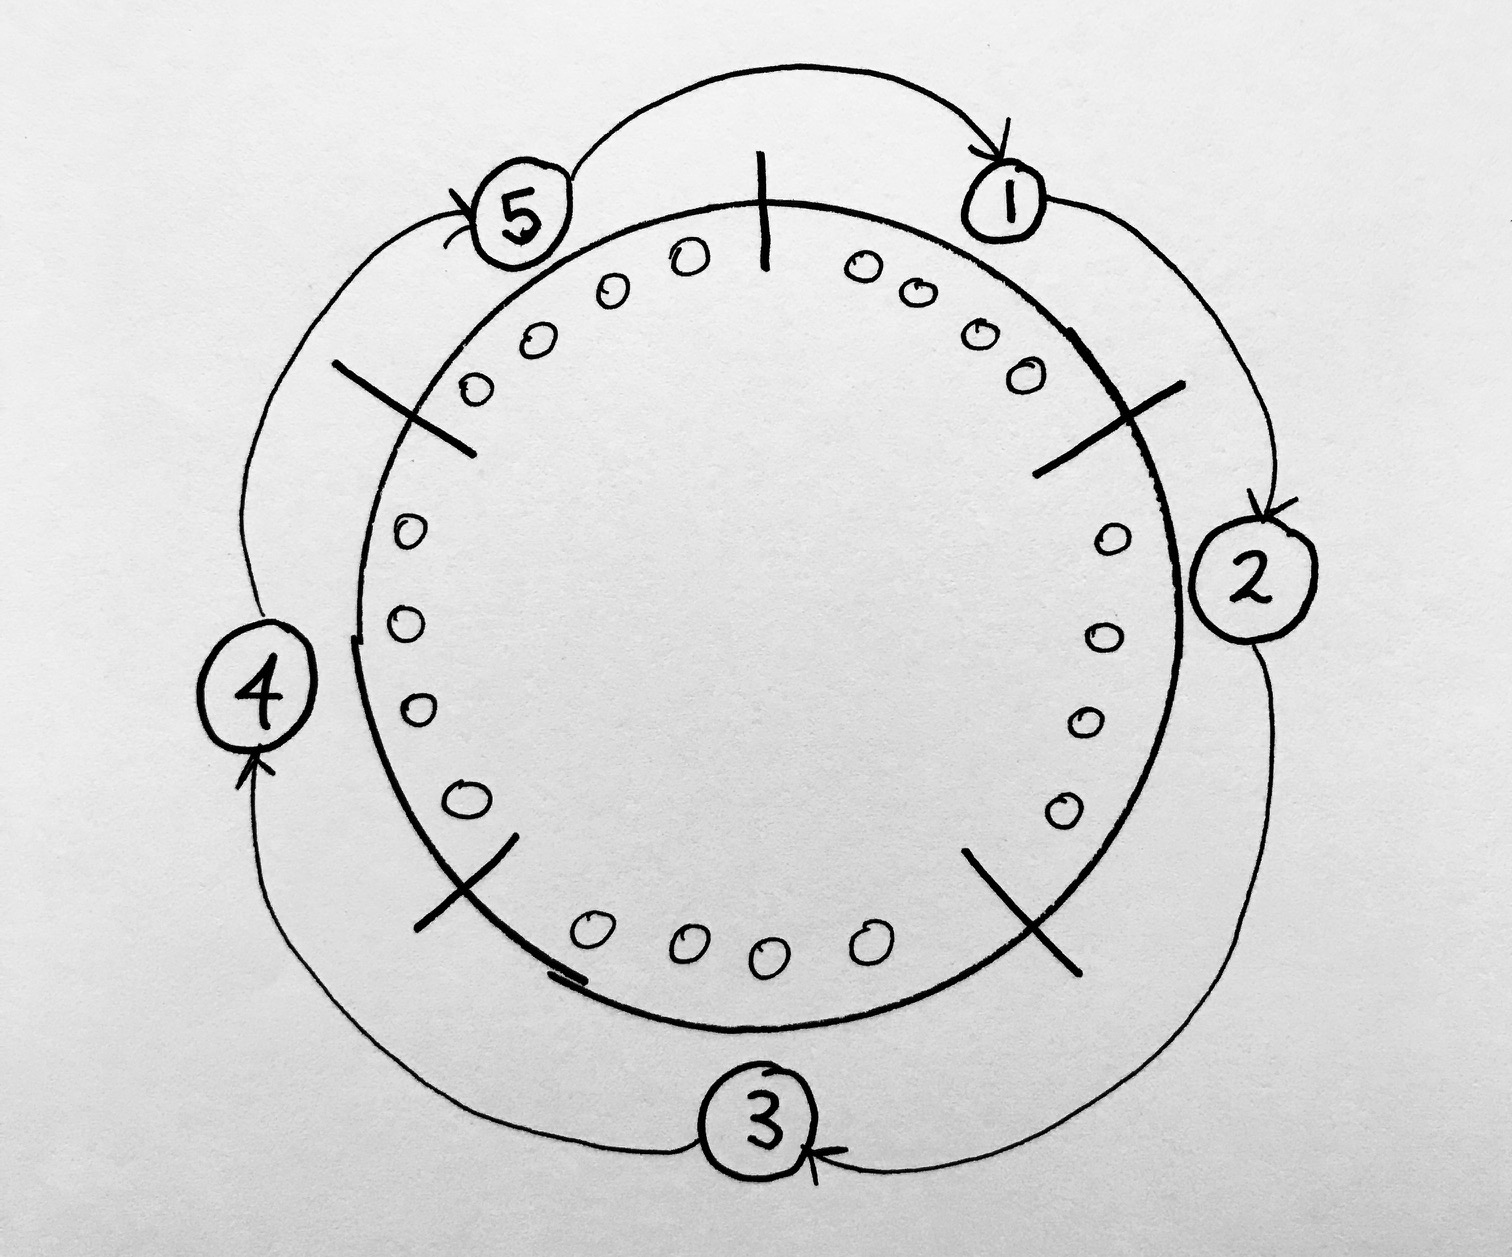
\includegraphics[width=0.5\textwidth]{fig/giant_step_ring.png}
    \caption{$5$ giant steps around a ring of $20$ proxies}

    \label{fig:giantstepring}
\end{figure*}
%%%%%%%%%%%%%%%%%%%%%%%%%%%%%%%%%%%%%%%%%%%%%%%%%%%%%%%%%%%%%%%%%%%%%%

Some number of proxies are less likely to be selected as step $g$ moves. For example, the proxies in previous selections left behind are referred to as \emph{needles} because they are hidden from the current selection. Additionally, proxies that have a lower chance of appearing in the random selection, e.g., the last few distinct proxies to be selected, have a lower probability of appearing in any selection. As $g$ moves, it also unbalances the load on proxies thereby increasing the number of selections that the censor must perform because there are more duplicate selections (misses).
\section{Coupon Collector Ring}

One may find a parallel between the Coupon Collector Problem \ac{CCP} and the problem of a censor who collects, not coupons, but proxies. Consider both the coupon and proxy as objects in some vast space, where all of these objects have the same chance of being selected. Each object is replaced after it is selected so that any object may be selected multiple times. It is increasingly difficult to collect a distinct object because most objects are selected more than once. The rarest object is the one that occurs at the very end to complete the collection. The selection of this very last unique object ends the game, since only the selection of distinct objects counts towards progress in this problem.

We can frame the needle algorithm as a \ac{CCP} variant, we call this the \ac{CCP-R} variant. Suppose that the coupon collector organizes collections from several different neighbourhoods. Each neighbourhood distributes a different set of coupons, and each of the coupons in each set is distinct. The coupon collector needs to travel through all of the neighbourhoods (these are conveniently arranged in a ring). The collector can't magically move from place to place and does not zigzag from neighbourhood to neighbourhood. If the collector misses a coupon from the first neighbourhood, then he must wait until all of the other neighbourhoods are visited before returning to collect the missed coupon. The missed coupon is rarer than all of the previously collected coupons. It is also rarer than all future coupons up until the point at which the collector returns to the specific neighbourhood with the missed coupon.

In our \ac{CCP-R} variant, the reverse power of 2 choices gives the collector a decision to make; he selects 2 coupons at random. If he already has more of 1 coupon than the other, he must keep the coupon that is less rare, and return the rarer coupon back to the store in the current neighbourhood. 

There is an expected number of attempts $E[X]$ by the collector to collect $n$ distinct objects. This can be extended to a censor, whose problem it is to enumerate, or discover, all the proxies. We use $E[X]$ to analyze the amount of effort that it would take a censor, on average, to enumerate all proxies. To simplify this analysis, we do not consider the ratio of honest to malicious clients and, for now, assume there is one malicious client, the censor. Honest and malicious client rates are examined in Section \ref{sec:bystander}, bystanders.

The needle algorithm is partly randomized and partly deterministic. The uniform random selection of 2 proxies is randomized, and the reverse power of 2 choices is deterministic. In addition, the movement of the steps is also deterministic. Because the steps move clock-wise around the ring, proxies are enumerated randomly within deterministic batches. Moving the steps around the ring serves two functions; 1) by limiting the size of proxies in a step, it squeezes the number of possible proxies that a censor can enumerate in each assignment, and 2) some proxies are left behind. This makes it more difficult for the censor to enumerate a complete collection of proxies due to these rare proxies (not unlike needles in a haystack). Restricting the size of the sublists in a step tends towards a deterministic enumeration of all of the proxies, so one must take care to not set too many giant steps. 

In Figure \ref{fig:8ring}, we see how different step sizes affect the enumeration of proxies. With one-step, the enumeration time is the slowest, because the needle proxies must be discovered within the largest pool of size $n$. Enumeration time starts to decrease with 2-steps, because the needle proxies are more likely to be selected with a smaller pool size of $n/2$. The enumeration time decreases with each increase in giant step $g$. The algorithm only functions as expected up to $g=n/2$ where there are at least $2$ proxies for each step. If there is only a single proxy in each step, as shown in the bottom right corner, the proxies are enumerated one after the other in $n$ assignments, because our reverse power of 2 choices algorithm cannot function as intended. We therefore restrict the giant step size to $1>g\leq \frac{n}{2}$ so that the proxies are never enumerated in deterministic order.

%%%%%%%%%%%%%%%%%%%%%%%%%%%%%%%%%%%%%%%%%%%%%%%%%%%%%%%%%%%%%%%%%%%%%%
\begin{figure*}[h!]
\centering
     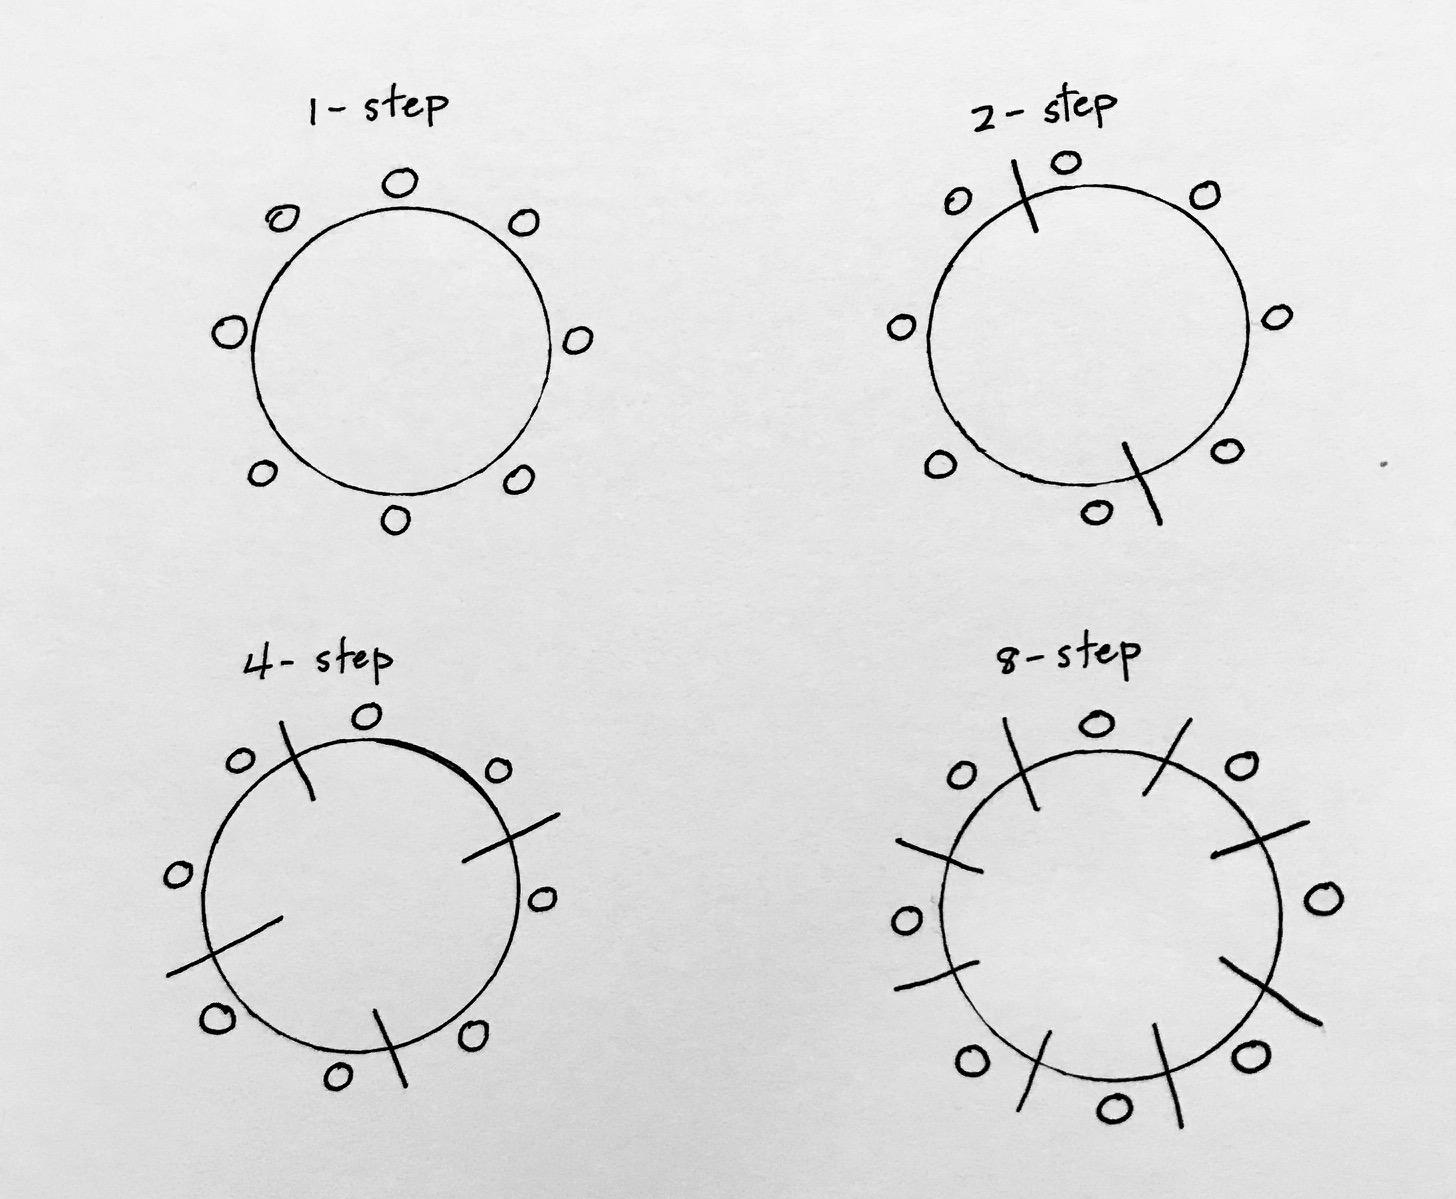
\includegraphics[width=0.5\textwidth]{fig/8_ring.png}
    \caption{Ring of 8 proxies with steps g=1,2,4,8}

    \label{fig:8ring}
\end{figure*}
%%%%%%%%%%%%%%%%%%%%%%%%%%%%%%%%%%%%%%%%%%%%%%%%%%%%%%%%%%%%%%%%%%%%%%
 
\section{Enumeration Analysis}
\label{sec:enum}

Recall that the enumeration of our collection of proxies occurs when the censor learns all of the proxies through assignment. The enumeration of proxies is modeled as the complete collection of coupons. The \ac{CCP-R} variant is used to calculate the average time to collect all distinct proxies.
 

\begin{table}[h]
  \centering
	\begin{tabular}{ll}
	\hline
	\cline{1-2}
	Parameter Name    & Description  \\
	\hline
    $n$     & total number of proxies \\
	$g$     & number of steps around a proxy ring  \\
	$s$     & size of proxies allocated in each step $n/g$ \\
    $H_n$   & harmonic number \\
    $px_i$  & the $i^{th}$ proxy \\
    $p_i$   & probability that the $i^{th}$ proxy is enumerated \\
    $p$     & sum probability that proxies $1$ to $n$ are enumerated \\
    $X_i$   & random variable of assignments to enumerate the $i^{th}$ proxy \\
    $X$     & random variable of sum of $X_i$ from $1$ to $n$ \\
    $E[X]$  & expected time on average to enumerate all proxies \\
	\hline
	\end{tabular}
  \caption{Notation used in the Enumeration Analysis}
  \label{tab:vars}
\end{table}

There are two different, yet intertwined, flavours of probabilities in our algorithm; the probability of \textit{selection} and the probability of \textit{choice}. The probability of selection is uniform random and is restricted by the size of the giant step $g$. When a pair of proxies is selected uniform randomly from the total collection of proxies, this is referred to as the selection. When we refer to likelihood of selection, we are talking about the probability of selection in relation to the coupon collector problem. Because we sample proxies randomly with replacement, a proxy can be selected twice in a pair. The probability of choice relates to the order in which a proxy is selected as a pair. The likelihood of choice is dependent on the load of a proxy as it affects the choice in the reverse power of 2 choices algorithm. Probability of choice is important in our analyses, particularly in the load balancing analysis.

\subsection{Algorithm Termination}

We define two lemmas below that we will use to approximate upper and lower bounds on the average enumeration time. We define the algorithm termination in terms of the rarest proxy, the last distinct proxy that is selected, $px_n$. Proxy $px_n$ has the probability of selection = $1/n$ making it the rarest proxy out of all of the other proxies. Note that this proxy must have load = 0 because it was never previously chosen out of a selected pair. Recall that the reverse power of 2 algorithm chooses the proxy with the highest load out of a pair of proxies. The rarest proxy can only be chosen if it is compared against itself. The only case where this occurs (when the proxy appears with probability of selection $1/n$) is when this proxy is selected in a pair. 

\begin{lemma}{A pair of the rarest proxy terminates the algorithm.}
\label{rarest}

Assume we have the rarest proxy \textbf{$px_n$} that has probability equal to $1/n$ of being selected in the reverse power of 2 choices algorithm. Suppose that this proxy is selected twice in a row and forms a pair. If the choice from this selected pair does not terminate the algorithm, there must be some other proxy in the collection of $n$ proxies that has not yet been chosen. If this statement is true, then proxy \textbf{$px_n$} must have a probability greater than $1/n$ and our initial assumption is false, leading us to a contradiction. Therefore, the proxy with probability $1/n$ terminates the algorithm if it is selected twice in a row, as a pair. In other words, the least likely, rarest proxy must occur as a pair for the algorithm to terminate. 
\end{lemma}

\begin{lemma}{The probability of enumerating the rarest proxy is at least $1/n^2$.}

By Lemma \ref{rarest}, the needle algorithm terminates after the rarest proxy is selected in a pair. The probability that the rarest proxy is selected is $1/n$. We sample with replacement, so the probability that the rarest proxy is selected twice in a pair, by counting argument, is $p=(\frac{1}{n})(\frac{1}{n}) = 1/n^2$.
\end{lemma}

\subsection{Upper Bound}  

We use the number of singletons described in Chapter \ref{sec:background}, $H_n$, directly to provide an upper bound on the average number of pairs selected, $E[X]$, before all of the proxies are enumerated. Singletons are proxies that occur only once and so have the lowest probability of selection. These proxies need to be paired with other proxies that have lighter loads to ensure that they are chosen by the reversed power of 2 choice algorithm. (They also need to appear as the first item in the pair for the tie-breaking logic.) Most of the singleton proxies occur at the end of the selection process, so the probability of selection for each of them is closer to $1/n$ than $n/n$. In the worst case (for the censor), all of the singleton proxies occur at the end of the collection. Since most of the proxies have load $> 1$ as $n$ increases, there is little chance that singleton proxies are chosen against non-singleton proxies, because most of these non-singleton proxies have appeared numerous times already and have higher assignment loads.

\begin{lemma}{The probability of collecting all of the singleton proxies is \\
$$\sum_{i=1}^{\lceil{H_n}\rceil} \bigg(\frac{i}{n^2}\bigg)$$}

The probability of collecting all of the singleton proxies is bounded above by the likelihood that the singleton proxies are selected in a pair with the rarest proxy $px_n$, the worst case for a censor. The rarest proxy $px_n$ is selected with probability $\frac{1}{n}$. The probability that some $i^{th}$ singleton proxy is selected in a pairing with $px_n$ is $p_i = (\frac{i}{n})(\frac{1}{n})$. 

If we pair all of the singleton proxies with the rarest singleton proxy, $px_n$, we get the probability pairs $(\frac{1}{n})(\frac{1}{n}) + (\frac{2}{n})(\frac{1}{n}) + ... + (\frac{H_n}{n})(\frac{1}{n})$. There is no guarantee that $H_n$ is an integer, indeed it will not be. Fractional pairings can't happen in our pairings, e.g. there is no half of a proxy selected. Because we are dealing with an upper bound, we say that the number of singleton proxies is $\leq \lceil{H_n}\rceil$. In addition, we need an even number of pairings, so $\lceil{H_n}\rceil$ is rounded to an even number. Generally stated, the probability of this pairing over all $H_n$ singletons is:

$$p \leq \sum_{i=1}^{\lceil{H_n}\rceil} \bigg(\frac{i}{n}\bigg) \bigg(\frac{1}{n}\bigg)$$
$$= \sum_{i=1}^{\lceil{H_n}\rceil} \bigg(\frac{i}{n^2}\bigg)$$

\end{lemma}

Now, we are ready to present the upper bound on the average number of assignments before all of the proxies are enumerated. Recall that $X_i$ is a random variable representing the number of assignments needed to enumerate the $i^{th}$ proxy, therefore $E[X_i]$ is the average number of assignments to collect the $i^{th}$ proxy. $E[X]$ is the average number of assignments needed to enumerate all of the proxies. We denote the $i^{th}$ proxy as $px_i$ where the last selected, rarest proxy is $px_{n}$ with probability $1/n$. The second rarest proxy is $px_{n-1}$ with probability $2/n$. The first proxy selected is $px_1$ with probability $1$.\\
 
\label{theorem:UBEX}
\begin{theorem} {Upper bound on $E[X] \leq \frac{n^2H_{\lceil{H_n}\rceil}}{g}$} 
\end{theorem}

\emph{Proof.} We use the probability of collecting all of the $H_n$ singleton proxies from Lemma $4$ to provide an upper bound on the average number of assignments needed to enumerate all of the proxies, $E[X]$. 

Like the classic CCP, this follows a geometric distribution, so $E[X_i] =\frac{1}{P_i}$. 

$$E[X_i] = 1/p_i = \frac{1}{\frac{i}{n^2}} = \frac{n^2}{i}$$

The expected number of assignments to find all $n$ proxies is bounded above by the sum of $E[X_1]$ to $E[X_n]$, where $n=\lceil{H_n}\rceil$:\\

$$E[X] \leq \sum_{i=1}^{\lceil{H_n}\rceil} \bigg(\frac{n^2}{i}\bigg)$$
$$E[X] = n^2 \sum_{i=1}^{\lceil{H_n}\rceil} \bigg(\frac{1}{i}\bigg)$$
$$E[X] = \bigg(n^2\bigg) \bigg(H_{\lceil{H_n}\rceil}\bigg)$$

When giant step $g$ is very small, the algorithm churns on a few proxies, meaning that a small proportion of proxies have high loads. By dividing $n$ proxies into $g>1$ giant steps, where each step has a sublist of size $s$, we make the algorithm more load balanced. In other words, the distribution of proxies in each step is smaller so the censor gets more chances to find the singletons.  We rework the upper bound to incorporate the number of giant steps $g$.

%%%%%%%%%%%%%%%%%%%%%%%%%%%%%%%%%%%%%%%%%%%%%%%%%%%%%%%%%%%%%%%%%%%%%%
\begin{figure*}[h!]
\centering
     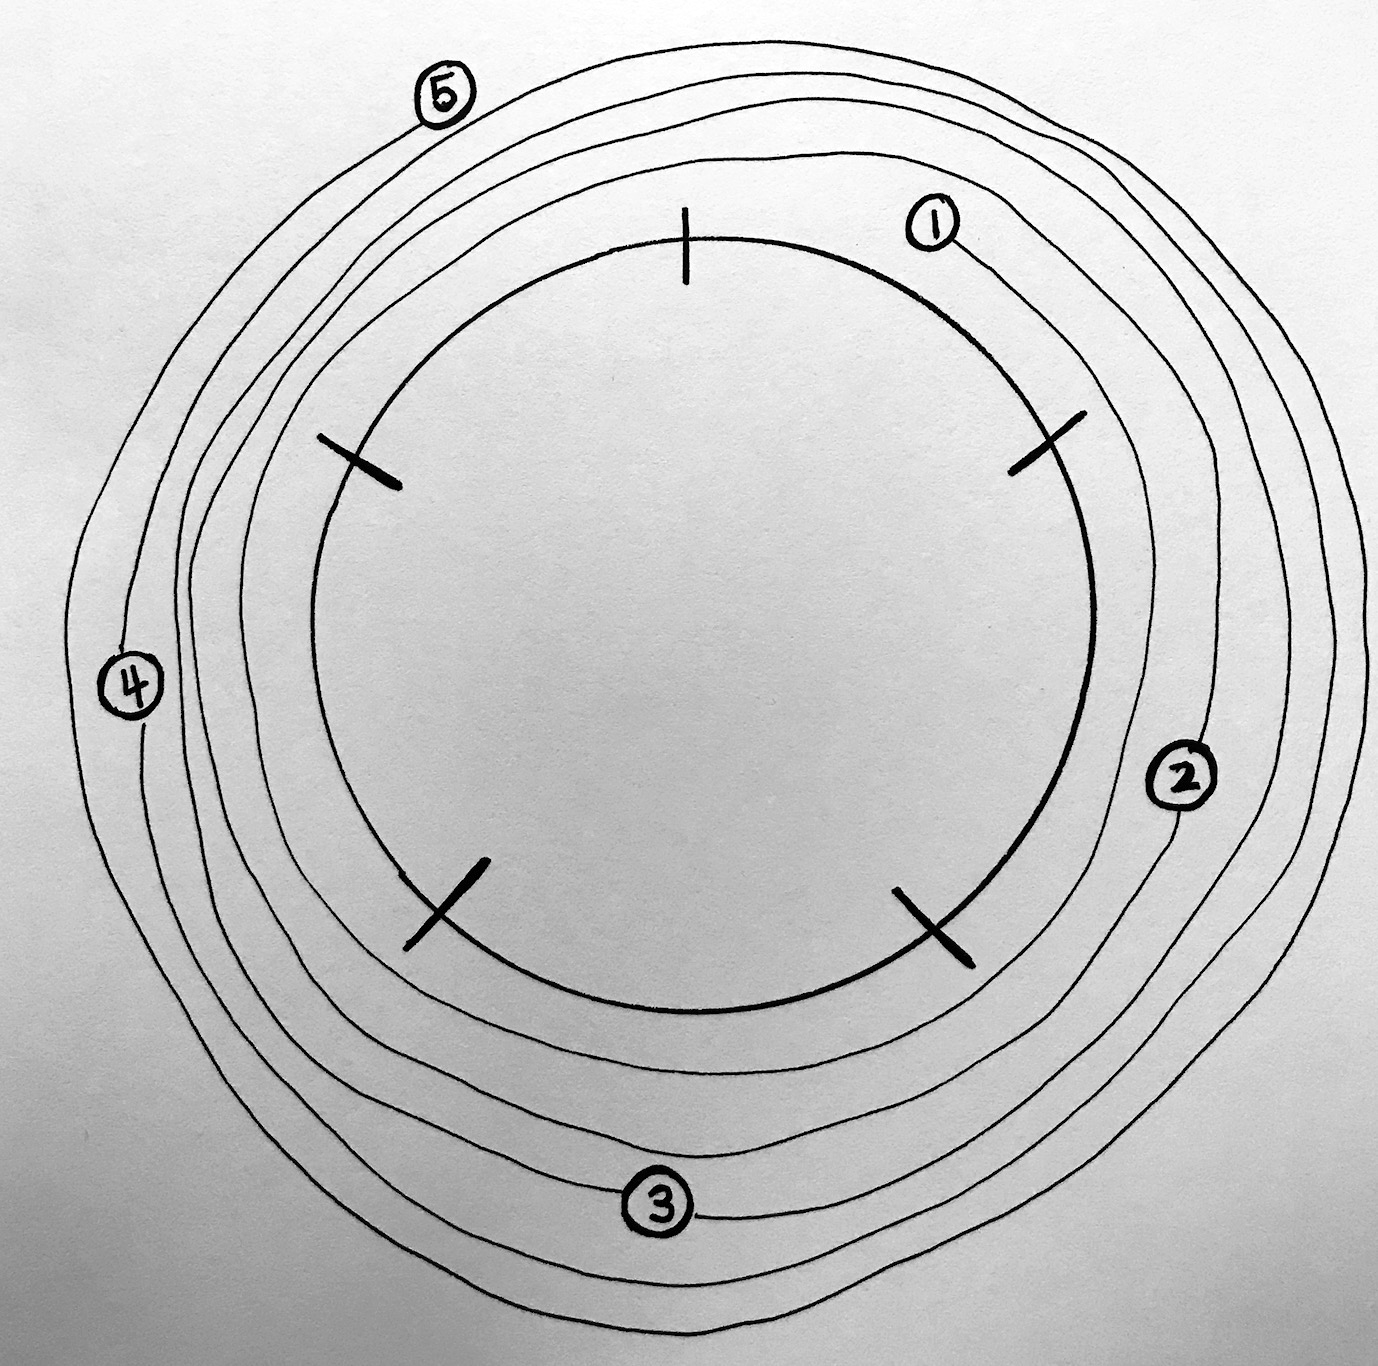
\includegraphics[width=0.5\textwidth]{fig/giant_step_upper_bound.png}
    \caption{Worst case enumeration in $5$ giant steps.}

    \label{fig:ubgs}
\end{figure*}
%%%%%%%%%%%%%%%%%%%%%%%%%%%%%%%%%%%%%%%%%%%%%%%%%%%%%%%%%%%%%%%%%%%%%%

We have $g$ giant steps and $H_n$ singleton proxies; $g$ divides the enumeration time into smaller sized sublists, making it proportionally easier for the censor to enumerate all $n$ proxies. In the worst case (for the censor), all of the singleton proxies are located in different steps, so all of the steps wait for the other steps' singletons to be enumerated before the algorithm can terminate. Figure \ref{fig:ubgs} shows a collection of proxies with $5$ giant steps. The first enumerated sublist occurs in the top right portion of the ring (denoted $(1)$). The algorithm proceeds clock-wise, moving through each sublist one by one. We divide the upper bound by the number of steps $g$ to obtain:

$$E[X] \leq \frac{ n^2H_{\lceil{H_n}\rceil}}{g}$$


\subsection{Lower Bound}
Before we present the lower bound on the average number of assignments before all of the proxies are enumerated, we consider the probability of singleton proxies that are very likely to be chosen. The reverse power of 2 choices relies on the load of the proxy in order to choose a proxy from a selected pair. Consider a singleton proxy that by definition has a lighter load because it is selected infrequently. When this proxy is paired with some other proxy with a higher probability of selection, the singleton proxy has \textit{less} chance to be chosen, because the proxy with the higher probability of selection has a higher chance of having more load. In other words, this singleton proxy has both a lower probability of selection and lower probability of choice. 

We concern ourselves with a lower bound, so we would like to know the type of scenario in which a singleton proxy has the higher probability of choice, meaning that the censor is able to enumerate proxies more easily. A singleton proxy paired with itself is guaranteed to be chosen and thus has the highest probability of choice out of any other pairing. We would like to know the probability of a pair of singleton proxies to appear.

\begin{lemma}{Singleton proxies occur in a pair with probability $p \geq \sum_{i=1}^{\lfloor{H_n}\rfloor} (\frac{i}{n})^2$}

% Maybe a bit confusing: 
% Another intuition is to consider the pairing of a singleton proxy with another, rarer singleton proxy because the rarer proxy most likely has a lighter load. This would also result in a high likelihood that the singleton proxy is chosen. However, the probability of selection of this proxy is smaller than the probability of a singleton proxy paired with itself, so it is not useful in developing our lower bound.

A repeated pair selection of the singleton proxies gives us the probability pairs $p=(\frac{1}{n})(\frac{1}{n}) + (\frac{2}{n})(\frac{2}{n}) + ... + (\frac{H_n}{n})(\frac{H_n}{n})$. The probability of the $i^{th}$ singleton proxy to be chosen is $(\frac{i}{n})^2$. The probability of this pairing for all $H_n$ singletons is:

$$p \geq \sum_{i=1}^{\lfloor{H_n}\rfloor} \bigg(\frac{i}{n}\bigg)^2$$

\end{lemma}
%%%%%%%%%%%%%%%%%%%%%%%%%%%%%%%%%%%%%%%%%%%%%%%%%%%%%%%%%%%%%%%%%%%%%%
\begin{figure*}[h!]
\centering
     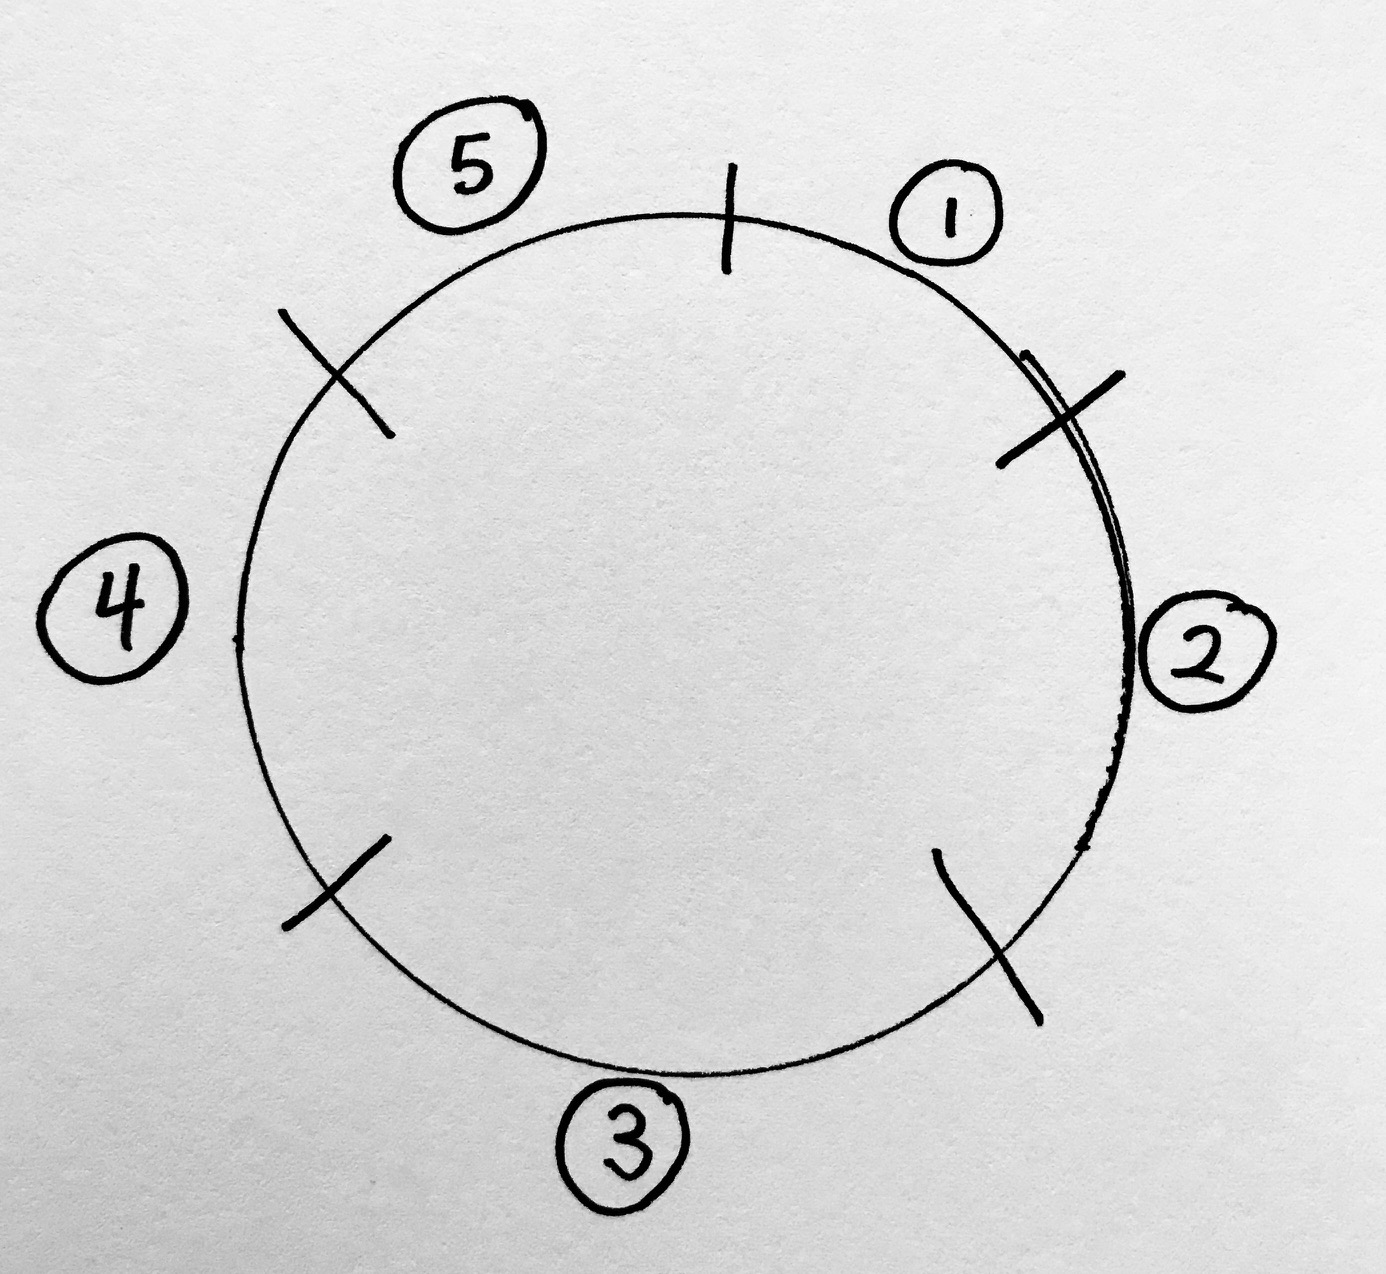
\includegraphics[width=0.5\textwidth]{fig/giant_step_lower_bound.png}
    \caption{Best case enumeration in $5$ giant steps.}

    \label{fig:lbgs}
\end{figure*}
%%%%%%%%%%%%%%%%%%%%%%%%%%%%%%%%%%%%%%%%%%%%%%%%%%%%%%%%%%%%%%%%%%%%%%


We use Lemma $6$ in the following proof to obtain the lower bound on $E[X]$. The fastest enumeration of all of the proxies is to collect all of the singleton proxies the first time that they show up in a randomly selected pair, that is, their very first selection. We again use $H_n$ singleton proxies, this time to bound the average number of assignments from below. We consider cases where $g\geq1$ and we change the variable $n$ to $s$ because we draw from $g$ sublists of size $s$. 

Returning to the idea of a ring of proxies, if all of the sublists are enumerated one directly after the other, none of the other steps are "held up" by any of the other previous steps. This means that there are no extra revolutions necessary to enumerate the steps, as shown in Figure \ref{fig:lbgs}.

%%%%%%%%%%%%%%%%%%%%%%%%%%%%%%%%%%%%%%%%%%%%%%%%%%%%%%%%%%%%%%%%%%%%%%
\begin{figure*}[h!]
\centering
     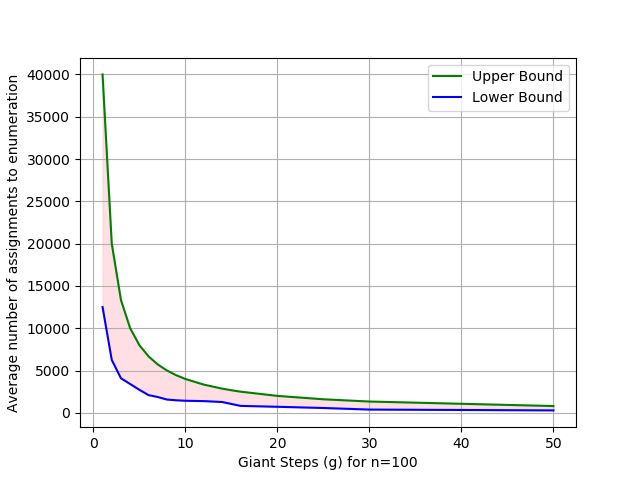
\includegraphics[width=1.0\textwidth]{fig/needle_expected_value_bounds.png}
    \caption{Upper and Lower Bounds for the Needle algorithm, where $n=100$, $g=1...50$}

    \label{fig:ublb}
\end{figure*}
%%%%%%%%%%%%%%%%%%%%%%%%%%%%%%%%%%%%%%%%%%%%%%%%%%%%%%%%%%%%%%%%%%%%%%

\label{theorem:LBEX}
\begin{theorem} {Lower bound on $E[X] \geq (g) (s^2)H^{(2)}_{\lfloor{H_n}\rfloor}$}
\end{theorem}

\emph{Proof.} Using the probability of pairs from Lemma $6$, we have a geometric distribution, so we can write: $$E[X_i] = \frac{1}{p_i} = \frac{1}{(\frac{i}{s})^2} = \bigg(\frac{s}{i}\bigg)^2$$

The expected number of assignments to find all $n$ proxies is bounded below by the sum of $E[X_1]$ to $E[X_n]$, where $n$ is the number of singleton proxies,$n=\lfloor{H_n}\rfloor$:\\

$$E[X] \geq \sum_{i=1}^{\lfloor{H_n}\rfloor} \bigg(\frac{s}{i}\bigg)^2$$
$$= s^2 \sum_{i=1}^{\lfloor{H_n}\rfloor} \frac{1}{i^2}$$
$$= s^2H^{(2)}_{\lfloor{H_n}\rfloor}$$\\

We have $g$ such enumerations of sublists with size $s$, one per each $g$ steps, therefore for all $n$ proxies are bounded from below by:

$$E[X] \geq (g)(s^2)H^{(2)}_{\lfloor{H_n}\rfloor}$$\\

In Figure \ref{fig:ublb}, we show the upper and lower bounds for $100$ proxies with giant steps 1 to 50. The enumeration time drops for each giant step, particularly dramatically where the giant step is increased from 1 to 2. It levels out as the giant step increases create a more deterministic enumeration. 

This concludes our discussion of bounds on the average number of assignments to enumerate all of the proxies in the needle algorithm. In the next section, we dive into a load balancing analysis to tell us more about how clients are assigned to proxies.

\label{sec:lb}
\section{Load Balancing Analysis}

We discussed maximum load as a metric for load balancing in Chapter \ref{sec:background}. We cannot guarantee that the number of bins (proxies) is equal to the number of balls (assignments), so the maximum load does not tell the whole picture. We need to look at the least loaded and heaviest loaded extremes and find an average measurement and compare this to the \textit{optimal load}. The optimal load is the load of each proxy if the system was perfectly balanced, that is, if the number of assignments were divided evenly over the number of proxies.

\begin{table}[h]
  \centering
	\begin{tabular}{ll}
	\hline
	\cline{1-2}
	Parameter Name    & Description  \\
	\hline
    $n$     & total number of proxies \\
    $m$     & total number of assignments in a series of trials \\
    $px_i$  & the $i^{th}$ proxy \\
    $p_i$   & probability that the $i^{th}$ proxy is enumerated \\
	$\ell$     & optimal load \\
	$u$     & maximum load \\
    $E[X]$  & expected time on average to enumerate all proxies \\
    $d_1$ & distance between $px_1$ and $px_{\frac{n}{2}}$ \\
    $d_2$ & distance between $px_{\frac{n}{2}}$ and $px_n$ \\
	\hline
	\end{tabular}
  \caption{Notation used in the Load Balancing Analysis}
  \label{tab:vars}
\end{table}

\begin{lemma}{Proxy loads increase linearly.}

We sort the proxies by their load, or their respective numbers of assignments, averaged over multiple trials. (Note that these are not static proxy numbers, but proxies that are numbered by their load.) We see that the loads have a linear relationship. This is because the probability of selection of the $px_i$ proxy decreases linearly from $i=1...n$. The probability of selecting the first proxy $px_1$ is $p_1=\frac{n}{n}=1$, the probability of the second $px_2$ is $p_2=\frac{n-1}{n}$, $p_{n-1}=2/n$, $p_{n}=1/n$, increasing linearly. This linear relationship between the probability of proxy selection is further reinforced by the probability of choice, where the maximum loaded proxy is always chosen over a lower load.
\end{lemma}

\begin{lemma}{The middle proxy, $px_{n/2}$, has the optimal load $\ell$.}

Let the number of total assignments in a series of trials be $m$, and $E[X]$ be the average number of assignments before all proxies are enumerated where $m>>E[X]$. The optimal load is $\ell=m/n$. Proxy $px_{n/2}$ has the probability of selection equal to $p_{\frac{n}{2}}=\frac{n/2}{n}$ in the reverse power of 2 choice selection. It is $n/2$ more likely to be chosen from the selection than proxies $px_1$ to $px_{\frac{n}{2} - 1}$ and $n/2$ less likely to be chosen over proxies $px_{\frac{n}{2} + 1}$. Its placement at the midway point of choice means that it is also at the midway point of the load $\ell$. 
\end{lemma}

\begin{theorem}{The maximum load, $u$, of proxy $px_1$ is twice as big as the optimal load, $2\ell$, if all of the proxies are enumerated.}

We know by CCP that the minimum load is at least $1$ if all of the proxies are enumerated. By Lemma $9$, we see that the middle proxy $px_{\frac{n}{2}}$ has the optimal load. Since the proxy load has a linear relationship by Lemma $8$, the distance, $d_1$ between $px_n$ and $px_{\frac{n}{2}}$ is equivalent to the distance, $d_2$ between $px_{\frac{n}{2}}$ and $px_1$. $px_{\frac{n}{2}}$ has the optimal load and the function is increasing linearly, therefore $px_{1}$ has twice the optimal load $u = 2\ell =(2)(\frac{m}{n})$.

\end{theorem}

\section{Bystander Analysis}
\label{sec:bystander}

We integrate honest users into our analysis where previously we only included the censor's problem of enumerating all of the proxies. We want to know the likelihood that a proxy has been assigned to an attacker, \textit{proxy exposure}, and the proportion of honest users, or \textit{bystanders}, that are affected by proxy exposure. We draw inferences from the load of each proxy and the probability that a client is an attacker to evaluate bystanders in section \ref{sec:bystandereval}.

\begin{table}[h]
  \centering
	\begin{tabular}{ll}
	\hline
	\cline{1-2}
	Parameter Name    & Description  \\
	\hline
    $p_a$       & probability that a client is an attacker\\
    $p_x$     & probability that a proxy is exposed \\
    $p_{nx}$     & probability that a proxy is not exposed \\
    $p_b$     & probability of bystander clients\\
	$h$     & historical load on a single proxy  \\
	$\ell$     & optimal load \\
	$m$     & maximum load \\

	\hline
	\end{tabular}
  \caption{Notation used in the Bystander Analysis}
  \label{tab:vars}
\end{table}

We define an \textit{exposed} proxy as a proxy that has at least one insider attacker assigned at any point in time. In a single assignment of a client to a proxy, the probability that the client is an attacker is given as $p_a$. The total number of assignments in a proxy is equivalent to its historical load $h$. 

\begin{lemma}{The probability that a proxy is not exposed is $(1-p_a)^{h}$.}

The number of client assignments that a proxy received is equal to the historical load $h$. The probability that all $h$ of these assignments are attackers is an "and" relationship. We multiply the probabilities of attackers per each assignment, $h$ times. Therefore, the probability that all of the assigned clients on a proxy are malicious is $(p_a)^h$. 

For a proxy to not be exposed, then it must never have had any attackers assigned to it. The probability that none of the clients assigned are attackers is $(1-p_a)^h$. Then the probability that a proxy is \textit{not} exposed is the same as the probability that none of the clients are attackers:

$$p_{nx} = (1-p_a)^h$$

\end{lemma}

%%%%%%%%%%%%%%%%%%%%%%%%%%%%%%%%%%%%%%%%%%%%%%%%%%%%%%%%%%%%%%%%%%%%%%
\begin{figure*}[h!]
\centering
     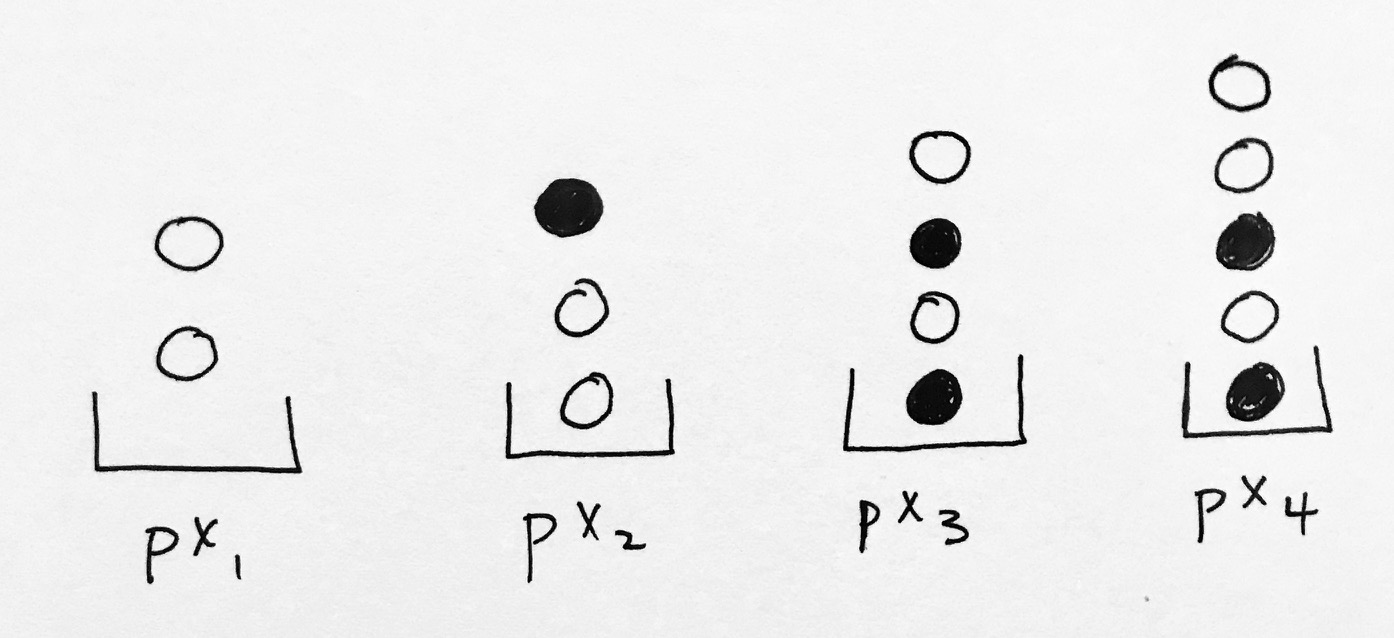
\includegraphics[width=0.5\textwidth]{fig/bystander_draw.png}
    \caption{Proxies $px_1$ to $px_4$ with honest and attacker clients.}

    \label{fig:bystandersdraw}
\end{figure*}
%%%%%%%%%%%%%%%%%%%%%%%%%%%%%%%%%%%%%%%%%%%%%%%%%%%%%%%%%%%%%%%%%%%%%%

We generalize the probability of exposure to apply to any proxy in the system using a bound on the maximum load. This is interesting for our bystander analysis because we observe that the probability that a proxy is exposed more closely approaches $100\%$ as the maximum load increases, thereby creating more bystanders.

\begin{lemma}{The probability that any proxy is exposed is $p_x \leq 1 - (1-p_a)^{m}$}

The height of any proxy must be less than or equal to the maximum height $m$ by definition. Without knowing the load on any individual proxy, we can say that the likelihood that an arbitrarily selected proxy is not exposed is less than or equal to the likelihood that the maximum loaded proxy is not exposed.
$$p_{nx} = (1-p_a)^{h} \leq (1-p_a)^{m}$$.

Conversely, the probability that any randomly selected proxy is exposed is less than or equal to the probability of exposure on the proxy that has the maximum load.

$$p_x = 1 - p_{nx}$$
$$ \leq 1 - (1-p_a)^{m}$$

\end{lemma}

The proxy that has the highest load has the highest chance of exposure. In Figure \ref{fig:bystandersdraw}, we give an example with four proxies, $px_1$ to $px_4$ that have attacker clients represented as filled circles, and honest clients shown as empty circles. There are no bystanders in proxy $px_1$ because it is not exposed. Proxies $px_2$ and $px_3$ both have two bystanders because they each have two honest clients and the proxies are exposed. There are three bystanders on proxy $px_4$. We've shown how the maximum load affects the probability of assigned attackers in a proxy, now we will compare the relationship of load balancing to bystanders. 
 


\begin{theorem}{The probability of bystanders on a proxy is $$p_b \leq (m)(1-p_a)(1-(1-p_a)^{m})$$}
\end{theorem}

\textit{Proof.} Honest clients occur with probability $1-p_a$ on any proxy. For an honest client to be considered a bystander, there must be at least one attacker assigned to the proxy. We consider the other attackers on a proxy as wasted resources on the part of the attacker.

We know from Lemma $12$ that the probability that any proxy is exposed is $p_x \leq 1 - (1-p_a)^{m}$. If $p_x = 0$ then there are no bystanders, because the proxy is not exposed. (In order for honest clients to be defined as bystanders, the proxy must be exposed by at least one attacker.) Therefore, we can say that the probability of bystanders on any proxy is less than the probability of bystanders on the proxy with the maximum load.

$$p_b \leq (m)(1-p_a)(1-(1-p_a)^{m})$$\\

We have shown that the amount of collateral damage, expressed by the probability of bystanders on a proxy, relies on the proxy load and the probability of attackers in each assignment. There are other interesting stories to tell about the impact of unbalancing proxy loads for proxy preservation. If we have a system that is perfectly balanced, with all proxy loads equal to $\ell$, intuitively we suspect that there will be more innocent bystanders $b$. We may reason that with lower proxy loads, such as those held in the needle algorithm of proxies $px_1$ to $px_{\frac{n}{2}-1}$, result in fewer bystanders because the likelihood of a malicious client attacker is reduced. We may also reason that in higher loaded proxies, there is more chance of proxy enumeration, but more wasted resources by the attacker. These musings are examined in Chapter \ref{sec:eval} through empirical data based on simulations of systems using the needle algorithm, uniform random distribution, power of 2 choices, and Tor's \texttt{bridgedb} proxy distribution strategy. 